% Magic comments - Informa ao compilador algumas regras de execução, como tipo de compilação ou codificação do texto
% !TeX root = monografia-aplicacao-redes-de-petri.tex
% !TeX encoding = UTF-8
% !BIB TS-program = XeLaTex
% !backend = biber

%% abtex2-modelo-trabalho-academico.tex, v-1.9.2 laurocesar
%% Copyright 2012-2014 by abnTeX2 group at http://abntex2.googlecode.com/
%%
%% This work may be distributed and/or modified under the
%% conditions of the LaTeX Project Public License, either version 1.3 of this license or (at your option) any later version.
%%
%% This work has the LPPL maintenance status `maintained'.
%%
%% INÍCIO DAS CUSTOMIZAÇÕES PARA A UNIVERSIDADE FEDERAL DE OURO PRETO%%

%% 2022.3.30 13h15 Danny Tonidandel
%% Altera as definições de capa, alterando  o comando, inserindo figuras próprias da Universidade e alterando a disposição dos elementos na contra-capa
%% Remove itens de abstract em francês
%% Altera disposição dos elementos na folha de aprovação
%% Altera o conteudo dos capítulos para um arquivo único.
%% Personalização do estilo biblatex-abnt para adequação à normaABNT 6023:2018
% Reseta contadores das notas de rodapé em cada capítulo
% Insere comandos para exibir uma caixa colorida de fundo cinza para notas explicativas, à escolha do autor

%% 2017.5.31 21h13 Danny Tonidandel
%% Altera nome de arquivo de logomarca
%% remove resumos em espanhol e italiano
%% Insere exemplos para elaboração de tabelas
%% Insere tabela de cronograma de atividades (para projeto de pesquisa)

%% FIM DAS CUSTOMIZAÇÕES PARA A UNIVERSIDADE FEDERAL DE OURO PRETO

%% This work consists of the files
% template-abnt-ufop-escola-de-minas.tex
% referencias.bib
%%
% --------------------------------------------
% ----------------------------------------------
% abnTeX2: Modelo de trabalho Academico (tese de doutorado, dissertacao de

% mestrado e trabalhos monograficos em geral) em conformidade com
% ABNT NBR 14724:2011: Informacao e documentacao - Trabalhos academicos -
% Apresentacao
% ------------------------------------------------------------------------
% ------------------------------------------------------------------------

\documentclass[
	% -- opções da classe memoir --
	12pt,				% tamanho da fonte
	openright,			% capítulos começam em pág ímpar (insere página vazia caso preciso)
	oneside,			% p/ impressão verso e anverso: twoside
	a4paper,			% tamanho do papel.
	% -- opções da classe abntex2 --
	%chapter=TITLE,		% títulos de capítulos convertidos em letras maiúsculas
	%section=TITLE,		% títulos de seções convertidos em letras maiúsculas
	%subsection=TITLE,	% títulos de subseções convertidos em letras maiúsculas
	%subsubsection=TITLE,% títulos de subsubseções convertidos em letras maiúsculas
	% -- opções do pacote babel --
	english,			% idioma adicional para hifenização
	brazil				% o último idioma é o principal do documento
	]{abntex2}

% ---
% Pacotes básicos
% ---

\usepackage{graphicx} 	% gráficos
\usepackage[table,xcdraw]{xcolor}	% tabelas
\graphicspath{{figuras/}} % pasta para figuras
\DeclareGraphicsExtensions{.pdf,.eps,.svg,.png,.jpg,.bmp}

\usepackage{indentfirst} % para identação no primeiro parágrafo
\usepackage{booktabs}
\usepackage{microtype} 	% justificação
\usepackage{verbatim}

% Pacotes de escrita matemática
\usepackage{amsmath,amssymb,unicode-math}


\usepackage{pdfpages} %  anexar pdf diretamente no documento
\usepackage{csquotes}

% Citações


% Opção 2: notas explicativas no sistema autor-data
\usepackage[backend=biber,
% % configuracoes do estilo abnt
 style=abnt,
 sccite, % sobrenomes em caixa alta
 ittitles, % Titulos em italico
 citecount, % contar o número de citações
 scbib, % biliografia em caixa alta
 justify, % alinhamento justificado
 noslsn,
 repeatfields,
 sorting=nty, % ordem alfabetica
 ]{biblatex}

% ARQUIVO COM AS REFERÊNCIAS BIBLIOGRAFICAS
\addbibresource{referencias.bib}

% ---
% Personalização do estilo biblatex-abnt
%Danny A. V. Tonidandel

% Adequa as urls de acordo com normas 6023:2018
\DeclareFieldFormat{url}{\bibstring{urlfrom}\addcolon\addspace \url{#1}}%
\DeclareFieldFormat{urldate}{\bibstring{urlseen}\addcolon\addspace #1}%

% Reseta contadores das notas de rodapé em cada capítulo
\makeatletter
\@addtoreset{footnote}{chapter}
\makeatother

% Pacotes adicionais - podem ser comentados
\usepackage{lipsum}	% para geração de texto aleatório
% ---

%Criação de Teoremas

% buscar documentação no CTAN
\newtheorem{exemplo}{Exemplo}
%\theoremstyle{break}

% ---
% Informações de dados para CAPA e FOLHA DE ROSTO
% ---
\titulo{DESENVOLVIMENTO DE UMA APLICAÇÃO WEB COM O OBJETIVO DE CONSTRUIR E SIMULAR REDES DE PETRI}
\autor{Douglas Meneses Barbosa}
\local{Ouro Preto}
\data{\the\year} % imprime o ano corrente no campo data
\orientador{Prof. Dr. Danny Augusto Vieira Tonidandel}
\coorientador{\color{red}Não definido}
\instituicao{Universidade Federal de Ouro Preto}
\tipotrabalho{Monografia de Graduação}
\preambulo{Trabalho apresentado ao Colegiado do Curso de Engenharia de Controle e Automação da Universidade Federal de Ouro Preto como parte dos requisitos para a obtenção do Grau de Engenheiro de Controle e Automação.}
% ---


% ---
% Aparência do PDF final

% alterando o aspecto da cor azul
\definecolor{blue}{RGB}{41,5,195}

% informações do PDF
\makeatletter
\hypersetup{
     	%pagebackref=true,
		pdftitle={\@title},
		pdfauthor={\@author},
    	pdfsubject={\imprimirpreambulo},
	    pdfcreator={LaTeX with abnTeX2},
		pdfkeywords={ufop}{latex}{decat}{monografia},
		colorlinks=true,   % opções: false, true
    	linkcolor=blue,    % cor de links internos
    	citecolor=blue,    % cor de links na bibliografia
    	filecolor=magenta, % color de links para arquivos
		urlcolor=blue,     % cor de hiperlinks (urls)
}
\makeatother
% ---

% ---
% Espaçamentos entre linhas e parágrafos
% ---

\setlength{\parindent}{1.3cm} % Tamanho do parágrafo


\setlength{\parskip}{0.2cm} % Espaçamento entre parágrafos
% tente também \onelineskip


\makeindex % compila o indice


\begin{document} % Início do documento

\frenchspacing % Retira espaço obsoleto

% Pré-TextualEXTUAIS
% \pretextual

% Capa - obrigatório

\begin{capa}
	\thispagestyle{empty}
		\centering
	\begin{center}
		\begin{minipage}{1\linewidth}
			\centering
			\begin{tabular}{ccc}
				\begin{tabular}{c}
					\\
					
\includegraphics[width=0.9cm]{logo-universidade.jpg}
				\end{tabular}
				&
				\begin{tabular}{c}
					\\
					{\large \imprimirinstituicao} \\
					{\large Escola de Minas} \\
					{\large CECAU - Colegiado do Curso de } \\
					{\large Engenharia de Controle e Automação}
				\end{tabular}
				&
				\begin{tabular}{c}
					\\
					
\includegraphics[width=2.1cm]{logo-unidade-2.jpg}
				\end{tabular}
			\end{tabular}
		\end{minipage}

\centering
\vspace*{1cm}
{\ABNTEXchapterfont\large\imprimirautor}
\vspace*{\fill}

{\ABNTEXchapterfont\bfseries \large \imprimirtitulo}
\vspace*{\fill}

{\large\imprimirtipotrabalho}
\vspace*{\fill}

{\large\imprimirlocal}, {\large \the\year}
%\par
\vspace*{1cm}
	\end{center}
\end{capa}



% Folha de rosto [OBRIGATÓRIO]
\imprimirfolhaderosto
% \imprimirfolhaderosto* se quiser ficha catalográfica

% Ficha bibliográfica [OPCIONAL,segundo determinação CECAU  e DECAT, 29/03/2023]
% \begin{fichacatalografica}
%     \includepdf{fig_ficha_catalografica.pdf}
% \end{fichacatalografica}


% Folha de aprovação - Obrigatório NBR 14724/2011
\begin{folhadeaprovacao}
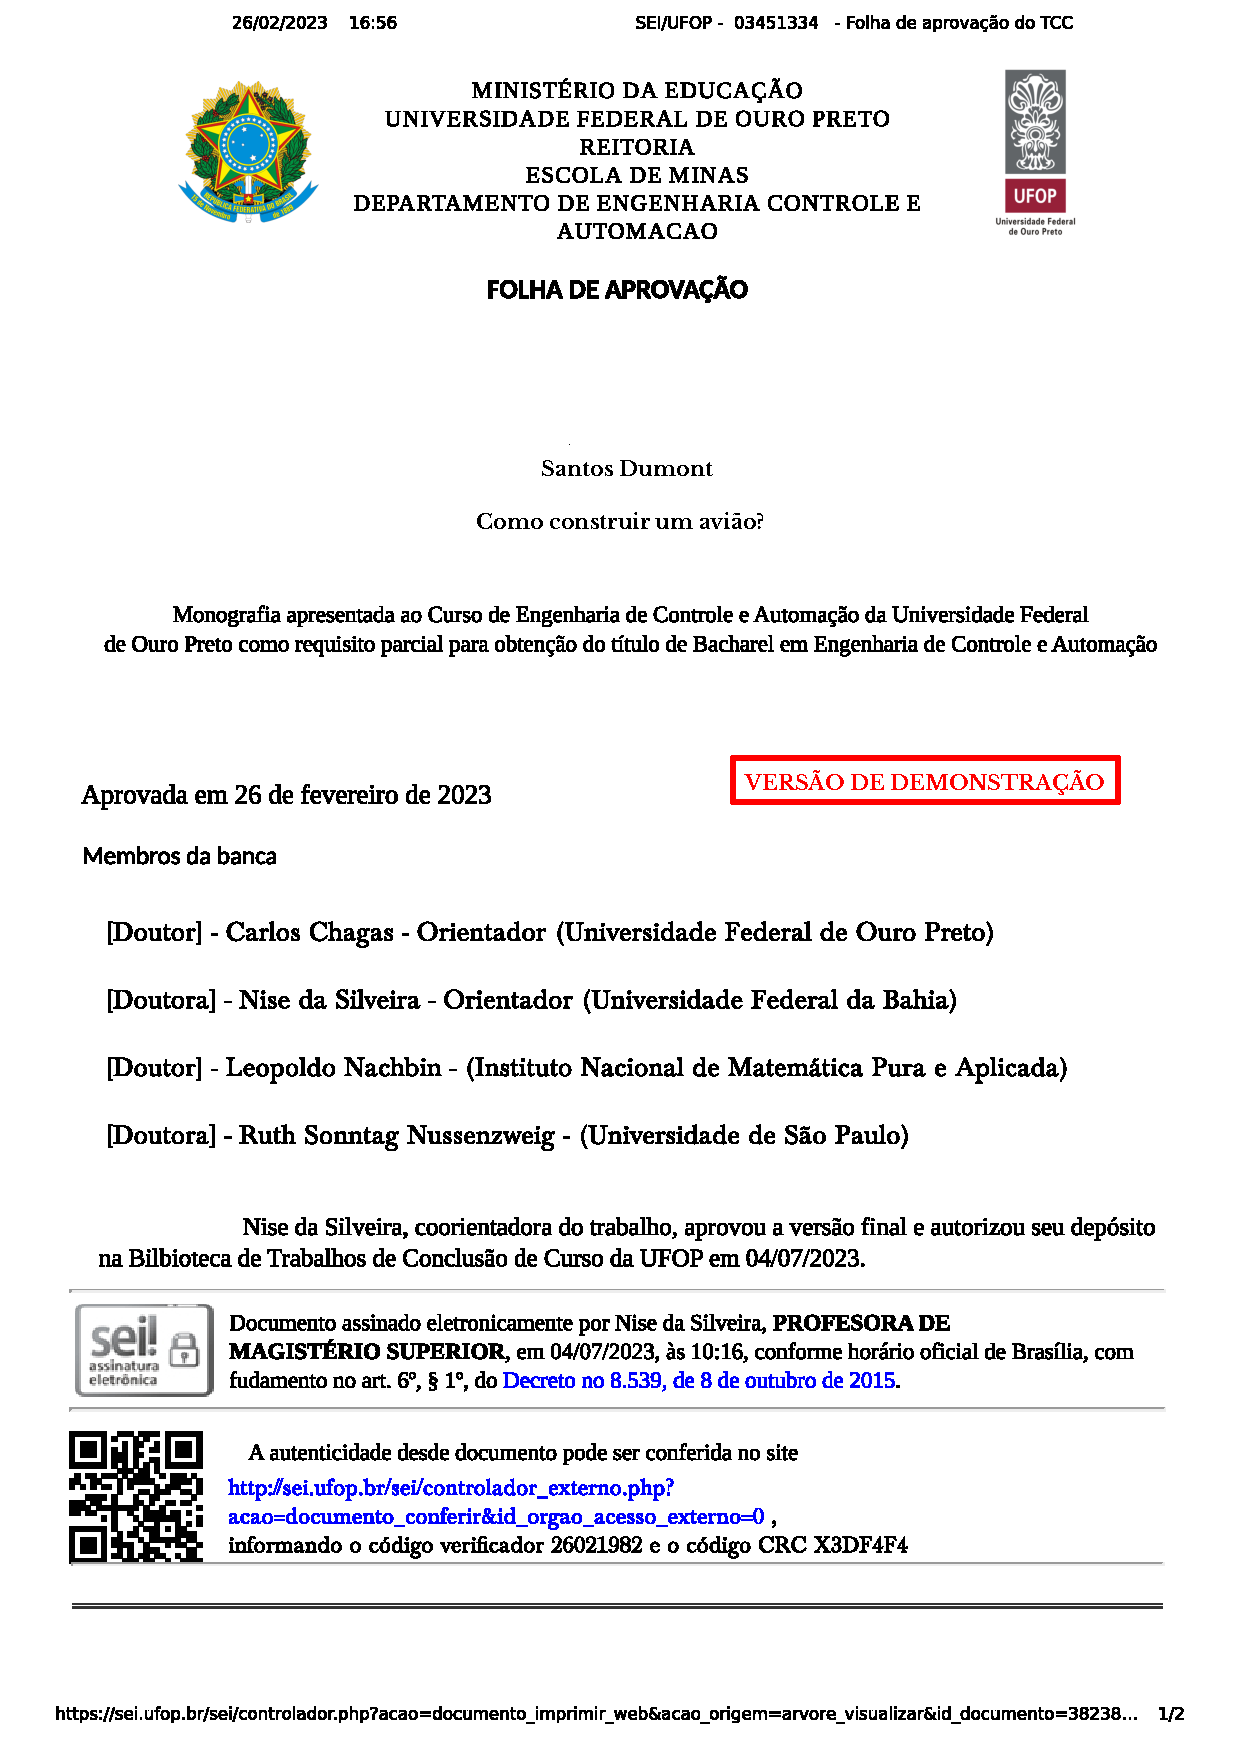
\includepdf{folha-de-aprovacao.pdf}
\end{folhadeaprovacao}


% Agradecimentos - opcional
\begin{agradecimentos}
\noindent Os agradecimentos [são opcionais, e] vem aqui... 
\end{agradecimentos}

% Epígrafe - Opcional
\begin{epigrafe}
    \vspace*{\fill}
\epigraph{\textsl{Júpiter leva 4332 dias para fazer uma revolução.}}{---~Oliver Lodge.}
\end{epigrafe}
% ---

% ---
% RESUMOS
% ---

% resumo em português
\setlength{\absparsep}{18pt} % ajusta o espaçamento dos parágrafos do resumo
\begin{resumo}
 \noindent O resumo deve ressaltar o objetivo, o método, os resultados e as conclusões do documento. A ordem e a extensão
 destes itens dependem do tipo de resumo (informativo ou indicativo) e do tratamento que cada item recebe no documento original. O resumo deve ser precedido da referência do documento, com exceção do resumo inserido no
 próprio documento. (\ldots) As palavras-chave devem figurar logo abaixo do resumo, antecedidas da expressão Palavras-chave:, separadas entre si por
 ponto e finalizadas também por ponto.

 \textbf{Palavras-chaves}: latex. abntex. editoração de texto.
\end{resumo}

% resumo em inglês
\begin{resumo}[Abstract]
 \begin{otherlanguage*}{english}

\noindent This is the english abstract.

   \vspace{\onelineskip}

   \noindent
   \textbf{Key-words}: latex. abntex. text editoration.
 \end{otherlanguage*}
\end{resumo}


% Lista de ilustrações
\pdfbookmark[0]{\listfigurename}{lof}
\listoffigures*
\cleardoublepage
% ---

% % inserir lista de tabelas
% \pdfbookmark[0]{\listtablename}{lot}
% \listoftables*
% \cleardoublepage
% % ---

% % ---
% % Lista de abreviaturas e siglas [OPCIONAL]
% % ---

% \begin{siglas}
%   \item[ABNT] Associação Brasileira de Normas Técnicas
%   \item[abnTeX] ABsurdas Normas para TeX
% \end{siglas}
% % ---

%---
% Lista de símbolos [OPCIONAL]
%---
% \begin{simbolos}
%   \item[$ \Gamma $] Letra grega Gama
%   \item[$ \Lambda $] Lambda
%   \item[$ \zeta $] Letra grega minúscula zeta
%   \item[$ \in $] Pertence
% \end{simbolos}
% ---

% ---
% Sumário
% ---
\pdfbookmark[0]{\contentsname}{toc}
\tableofcontents*
\cleardoublepage


% Reinicia contadores das notas de rodapé
\makeatletter
\@addtoreset{footnote}{chapter}
\makeatother



% ELEMENTOS TEXTUAIS

\textual

% Modelo de capitulo com a introducao, objetivos e estrutura do texto

% --
\chapter[Introdução]{Introdução}

nome da aplicação: Online Petri Net Simulator

Em 1962, Carl Adam Petri, por meio de sua dissertação, mostrou para o mundo a sua criação, as redes de Petri \cite{petri1962kommunikation}. Podemos definir uma rede de Petri como sendo uma ferramenta matemática para modelagem de sistemas concorrentes. Além da modelagem matemática, as redes de Petri podem ser ilustradas graficamente por meio de seus elementos, os lugares, as transições e os arcos. Além disso, com a evolução da industria e da tecnologia, as redes de Petri ganharam ainda mais relevância, uma vez que elas permitem a modelagem de diversos tipos de sistemas, em diferentes áreas. 

A evolução da industria e da tecnologia também culminou com a popularização da internet \cite{lins2013evoluccao}. O surgimento do World Wide Web, em 1990, por Tim Berners-Lee, permitiu aos primeiros usuários da internet, como conhecemos hoje, a interação com um sistema de hipertexto. Com o passar dos anos, as aplicações web se tornaram cada vez mais comuns e sofisticadas. O que antes começou com páginas estáticas evoluiu para aplicações dinâmicas, interativas e de fácil acesso para a maioria das pessoas. Atualmente, se consegue ter uma experiência muito próxima as funcionalidades de um computador pessoal, com aplicações desktop, apenas manipulando abas em um navegador.

Diante da facilidade de acesso a aplicativos web por meio dos navegadores, como Google Chrome, Firefox, Safari, Edge, entre outros, surge a seguinte ideia: desenvolver uma aplicação web que possibilite aos usuários a criação e simulação do comportamento de redes de Petri, de forma simples e intuitiva. Para tal, torna-se necessário o conhecimento de tecnologias voltadas para o desenvolvimento web, como HTML5, CSS3 e JavaScript.

Além do conhecimento em desenvolvimento, será necessário  compreender os conceitos e práticas de infraestrutura, viabilizando a disponibilidade e o acesso contínuo à aplicação web. Uma vez desenvolvida, a aplicação pode ser disponibilizada para acesso por qualquer usuário que possua conexão com a internet, facilitando a modelagem de redes de Petri.

% \textcolor{red}{Abordar mais argumentos e concatenar melhor as ideias trazidas nos parágrafos}


% Este documento e seu código-fonte são exemplos de referência de uso da classe \textsf{abntex2} e do pacote \textsf{biblatex-abnt}. O documento exemplifica uma realização possível entre as opções existentes na norma ABNT NBR 10520:2018 \emph{Citações em documentos -- Apresentação} e da norma ABNT NBR 6023:2018 \emph{Referências -- Elaboração}, cientes de que existe uma distância entre as ``normas'' e a interpretação das normas. Assim, antes de tudo, converse com seu orientador ou representantes do programa de pós-graduação de sua universidade, mostre uma cópia do documento PDF gerado por este arquivo e certifique-se de que não terá problemas futuros com relação à aceitação ou não do modelo.

\section{Justificativas e Relevância}

As redes de Petri representam uma poderosa ferramenta gráfica e matemática para a modelagem e análise de sistemas concorrentes e distribuídos. No entanto, o seu entendimento pode ser um desafio, especialmente para aqueles sem familiaridade com os conceitos e experiência matemática.

Atualmente, existem algumas ferramentas capazes de construir e simular redes de Petri. Entretanto, muitas delas requerem um conhecimento mínimo de computação, para que possam ser instaladas em sistemas operacionais como Linux, Windows e MacOS. Além disso, algumas delas não são multiplataforma, restringindo o acesso dessas ferramentas pelas pessoas.

Nesse contexto, uma aplicação web, simples e intuitiva, atenderia as necessidades, tanto de usuários comuns, como o de estudantes e pesquisadores interessados em entender o funcionamento das redes de Petri. Através de uma aplicação web, o acesso é simplificado e facilitado, pois elimina a necessidade de instalações complicadas e pré-conhecimento técnico avançado.



% Um exemplo de citação em linha pode ser visto como em \textcite{Einstein1920}.

% Um exemplo de citação do tipo autor-data pode também ser elaborado \cite{Einstein1920}.

% Um exemplo de citação em nota de de rodapé, com notas explicativas pode ser visto aqui.\footcite[Esta nota vem antes.][p.~22]{descartes-carta-mersene}

% Um outra outra forma de citação em nota explicativa pode ser elaborada\footnote{Escreva sua nota explicativa aqui, conforme \textcite{boyle1772}.}

% \section{Materiais e Métodos}
% Uma estrutura de tópicos é muito comum em metodologias. Uma forma de fazê-lo é utilizando o comando ``itemize'':

% \begin{itemize}
% 	\item Tópico 1;
% 	\item Tópico 2;
% 	\item etc.
% \end{itemize}

% Se preferir itens numerados, utilizar o ambiente ``Enumerate'':
%     \begin{enumerate}
% 	\item Tópico 1;
% 	\item Tópico 2.
%     \end{enumerate}

\section{Objetivo Geral}

O desenvolvimento de uma aplicação web capaz de criar e simular o comportamento de redes de Petri.

\section{Objetivos Específicos}

\begin{itemize}
        \item Desenvolvimento de um motor de simulação, capaz de simular o comportamento das redes de Petri criadas, possibilitando a visualização, por parte do usuário, do comportamento em diferentes cenários;
        \item Desenvolvimento de uma interface simples e intuitiva; 
	\item Aprendizado de tecnologias voltadas para o desenvolvimento web; 
	\item Criação de uma alternativa simples e de fácil acesso para o aprendizado de redes de Petri;
        \item Alocação da aplicação em um servidor, permitindo o acesso público.
\end{itemize}


\section{Metodologia}

% \textcolor{red}{Explicação sobre o ciclo de desenvolvimento de software: requisitos, design, desenvolver, testar e implementar}

Inicialmente, para o desenvolvimento da aplicação web, capaz de construir e simular o comportamento de redes de Petri, será necessário entender os requisitos e características mínimas para o funcionamento da aplicação. Analisando softwares já existentes que cumprem essa função, serão desenvolvidas as seguintes funcionalidades básicas:

\begin{itemize}
        \item Área da tela em que a rede de Petri será renderizada;
        \item Botões para inserção de lugares, arcos, tokens e transições;
        \item Botão de simulação em que, ao ser acionado, irá permitir a análise do comportamento da rede de Petri criada;
        \item Opção de definir labels para os lugares, arcos e posições;
        \item Alteração de cor da transição quando houver os requisitos mínimos satisfeitos;
        \item Opção de importação e exportação de projetos.
\end{itemize}

Com as características básicas da aplicação definidas, será desenvolvido um diagrama de fluxo, ilustrado na figura \ref{fig:diagrama_fluxo}, evidenciando o passo a passo de funcionamento da aplicação. 

\begin{figure}[ht] 
	\centering
	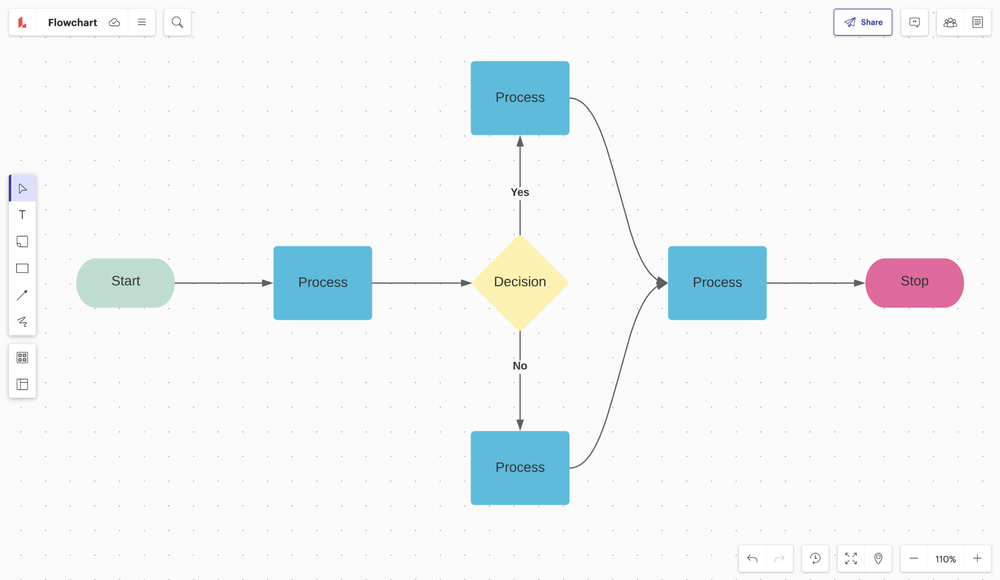
\includegraphics[scale=0.4]{exemplo_diagrama_de_fluxo.png}
	\caption[Exemplo de diagrama de fluxo]{Diagrama de fluxo. Fonte: \textcite{boyle1772}.}
	\label{fig:diagrama_fluxo}
\end{figure}

Paralelamente ao desenvolvimento do diagrama de fluxo, será criado um diagrama de classe \ref{fig:diagrama_classe}, definindo as diferentes classes de objetos que serão utilizados.

\begin{figure}[ht] 
	\centering
	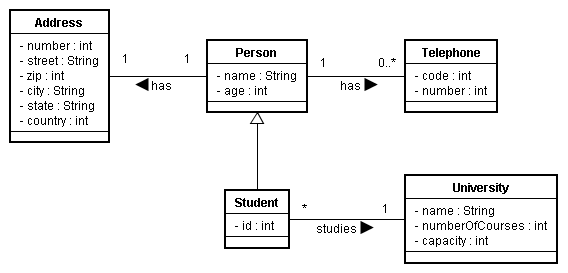
\includegraphics[scale=0.6]{exemplo_diagrama_de_classe.png}
	\caption[Exemplo de diagrama de classe]{Diagrama de classe. Fonte: \textcite{boyle1772}.}
	\label{fig:diagrama_classe}
\end{figure}

\newpage

Após a definição do design, com a criação do diagrama de fluxo e do diagrama de classe, inicia-se o processo de programação. A linguagem de programação JavaScript será utilizada, juntamente com HTML e CSS. O desenvolvimento acompanhará o design pré-estabelecido. Com isso, espera-se a criação de um MVP (Minimum Viable Product).

Com a criação do MVP, em um ambiente local, a aplicação será hospedada em um servidor on-premisse da Universidade Federal de Ouro Preto. Após a hospedagem, espera-se que a aplicação esteja disponível para acesso público por meio da internet.


%link da imagem diagrama de fluxo: https://cdn-cashy-static-assets.lucidchart.com/marketing/pages/lucidspark/consideration/brainstorm-to-identify-each-part-of-your-workflow@2x@2x.png

% \textcolor{red}{Criar diagrama de fluxo com redes de Petri}

% Além do diagrama de fluxo, é necessária a criação de um diagrama de classe \ref{fig:diagrama_classe}. No diagrama de classe, define-se as diferentes classes de objeto que serão utilizados na aplicação. 

%Link da imagem diagrama de classe: https://www.researchgate.net/publication/228951230/figure/fig10/AS:349293408997379@1460289446190/Figura-11-Diagrama-de-classes-da-aplicacao-O-modelo-exibido-na-Figura-11-pode-ser-criado.png

% \textcolor{red}{Caso seja criado um banco de dados, explicar o seu funcionamento aqui}

% \textcolor{red}{Figuras de exemplo, substituir por imagem de melhor qualidade. Se possível, criar as próprias imagens}

%Falar sobre manuntenção da aplicação
%Falar sobre o estudo de softwares já existem

% \textcolor{red}{Novos tópicos serão abordados na metodologia. Muitas abordagens ainda não foram definidas. Ao longo do desenvolvimento, elas se tornarão mais claras }


% \section{Organização e estrutura}

% A estrutura e organização deve apresentar os assuntos abordados ao longo do seu texto. Por exemplo, no capítulo \ref{cap:revisao-de-literatura} são apresentados e discutidos os principais trabalhos neste campo de pesquisa. Já no capítulo \ref{cap:desenvolvimento}, que, por acaso, começa na página \pageref{cap:desenvolvimento}, o trabalho é desenvolvido.

% Um exemplo de tabela é apresentada na tabela~\ref{tab:001}. Você pode elaborar também tabelas online ou a partir de qualquer planilha eletrônica, inclusive em outros estilos, gerando o código em \LaTeX. Após isso, basta copiar e colar o código aqui. Um exemplo de site é o ``Tables Generator'': \url{http://www.tablesgenerator.com/}.

% % Please add the following required packages to your document preamble:
% % If you use beamer only pass "xcolor=table" option, i.e. \documentclass[xcolor=table]{beamer}
% \begin{table}[h]
% \centering
% \caption{Uma tabela}
% \label{tab:001}
% \resizebox{0.5\textwidth}{!}{%
% \begin{tabular}{|l|llllllllll|}
% \hline
%                                    & \multicolumn{10}{l|}{\cellcolor[HTML]{FF0000}\textbf{Meses}}                                                                                                                                                                         \\ \hline
% \cellcolor[HTML]{5EB91E}           & \multicolumn{1}{l|}{1} & \multicolumn{1}{l|}{2} & \multicolumn{1}{l|}{3} & \multicolumn{1}{l|}{4} & \multicolumn{1}{l|}{5} & \multicolumn{1}{l|}{6} & \multicolumn{1}{l|}{7}  & \multicolumn{1}{l|}{8} & \multicolumn{1}{l|}{9} & 10 \\ \hline
% \cellcolor[HTML]{5EB91E}\textbf{1} & \multicolumn{1}{l|}{}  & \multicolumn{1}{l|}{x} & \multicolumn{1}{l|}{}  & \multicolumn{1}{l|}{}  & \multicolumn{1}{l|}{}  & \multicolumn{1}{l|}{}  & \multicolumn{1}{l|}{}   & \multicolumn{1}{l|}{}  & \multicolumn{1}{l|}{}  &    \\ \hline
% \cellcolor[HTML]{5EB91E}\textbf{2} & \multicolumn{1}{l|}{x} & \multicolumn{1}{l|}{x} & \multicolumn{1}{l|}{}  & \multicolumn{1}{l|}{}  & \multicolumn{1}{l|}{}  & \multicolumn{1}{l|}{}  & \multicolumn{1}{l|}{xx} & \multicolumn{1}{l|}{}  & \multicolumn{1}{l|}{}  & x  \\ \hline
% \cellcolor[HTML]{5EB91E}\textbf{3} & \multicolumn{1}{l|}{}  & \multicolumn{1}{l|}{x} & \multicolumn{1}{l|}{}  & \multicolumn{1}{l|}{x} & \multicolumn{1}{l|}{}  & \multicolumn{1}{l|}{}  & \multicolumn{1}{l|}{}   & \multicolumn{1}{l|}{}  & \multicolumn{1}{l|}{}  &    \\ \hline
% \cellcolor[HTML]{5EB91E}\textbf{4} & \multicolumn{1}{l|}{}  & \multicolumn{1}{l|}{}  & \multicolumn{1}{l|}{}  & \multicolumn{1}{l|}{x} & \multicolumn{1}{l|}{}  & \multicolumn{1}{l|}{}  & \multicolumn{1}{l|}{xx} & \multicolumn{1}{l|}{}  & \multicolumn{1}{l|}{}  &    \\ \hline
% \cellcolor[HTML]{5EB91E}\textbf{5} & \multicolumn{1}{l|}{}  & \multicolumn{1}{l|}{}  & \multicolumn{1}{l|}{}  & \multicolumn{1}{l|}{}  & \multicolumn{1}{l|}{}  & \multicolumn{1}{l|}{}  & \multicolumn{1}{l|}{}   & \multicolumn{1}{l|}{}  & \multicolumn{1}{l|}{}  &    \\ \hline
% \cellcolor[HTML]{5EB91E}\textbf{6} & \multicolumn{1}{l|}{}  & \multicolumn{1}{l|}{}  & \multicolumn{1}{l|}{}  & \multicolumn{1}{l|}{}  & \multicolumn{1}{l|}{}  & \multicolumn{1}{l|}{}  & \multicolumn{1}{l|}{xx} & \multicolumn{1}{l|}{}  & \multicolumn{1}{l|}{}  &    \\ \hline
% \end{tabular}%
% }
% \end{table}

% Capitulo de revisão de literatura

\chapter{Fundamentação teórica} \label{cap:revisao-de-literatura}

% Um capítulo de revisão de literatura, também chamado de revisão teórica ou bibliográfica pode ser desenvolvido aqui. Procure dissertar sobre os autores e trabalhos mais relevantes em seu campo de estudo, em um diálogo com sua proposta. Um exemplo de citação em linha pode ser visto como em \textcite{Einstein1920}. 

% Um exemplo de citação do tipo autor-data pode também ser elaborado \cite{Einstein1920}. 

% Um exemplo de citação em nota de de rodapé, com notas explicativas pode ser visto aqui.\footcite[Esta nota vem antes.][p.~22]{descartes-carta-mersene} 

% Um outra outra forma de citação em nota explicativa pode ser elaborada\footnote{Escreva sua nota explicativa aqui, conforme \textcite{boyle1772}.}

% Um exemplo de citação direta pode ser feito. Conforme aconselha \textcite{boyle1772-a}:

% \begin{citacao}
% 	(...) Nam dui ligula, fringilla a, euismod sodales, sollicitudin vel, wisi. Morbi auctor lorem non justo. Nam lacus libero, pretium at, lobortis vitae, ultricies et, tellus. Donec aliquet, tortor sed accumsan bibendum, erat ligula aliquet magna, vitae ornare odio metus a mi. Morbi ac orci et nisl hendrerit mollis. Suspendisse ut massa. Cras nec ante. Pellentesque a nulla. Cum sociis natoque penatibus et magnis dis parturient montes, nascetur ridiculus mus. Aliquam tincidunt urna. Nulla ullamcorper vestibulum turpis. Pellentesque cursus luctus mauris.(...)
% \end{citacao}

\section{Redes de Petri}

As redes de Petri surgiram por volta da década de 1960 pela mente de Carl Adam Petri. Em 1962, Petri apresentou sua tese intitulada ``Kommunikation mit Automaten'', em que descreveu pela primeira vez a estrutura e funcionamento das redes de Petri. Esse nova ideia de representar sistemas permitiu a análise de sistemas concorrentes e paralelos.

Com o passar dos anos, a evolução tecnológica durante a terceira revolução industrial \cite{coutinho1992terceira} evidenciou os benefícios das redes de Petri, e sua aplicabilidade foi ampliada para além da modelagem de processos industriais, sendo adotada também para descrever processos dentro das áreas de Ciência da Computação e Engenharia de Software. Sendo assim, a partir dos anos de 1980, com o crescimento da automação industrial, as redes de Petri começaram a ser adaptadas para atender as necessidades de diferentes áreas. Com isso, surgiram as redes de Petri coloridas, as redes de Petri temporizadas e as redes de Petri estocásticas, como principais exemplos. 

\subsection*{O básico de redes de Petri}

Segundo \cite{CassandrasLafortune08}, uma rede de Petri clássica é representada graficamente por lugares, transições e arcos. Os lugares representam os estados do sistema, as transições indicam os eventos ou ações que podem ocorrer durante o funcionamento do sistema. Os arcos direcionados conectam os lugares as transições e as transições aos lugares. Essa estrutura permite a análise de propriedades importantes dos sistemas, como alcançabilidade, vivacidade, deadlock, reversibilidade, entre outras propriedades fundamentais para analise do comportamento de sistemas complexos. 

As redes de Petri seguem uma lógica matemática. Sendo assim, seus elementos são definidos como sendo:

\begin{equation*}
    \centering
    \left( P, T, A, w \right) \,,
    \label{elementos_rede_petri}
\end{equation*}
em que 

\textbf{$P = \left \{ p_{1},p_{2},...,p_{n} \right \}$} é o conjunto de lugares;

$T = \left \{ t_{1},t_{2},...,t_{n} \right \}$ é o conjunto de transições;

$A \subseteq \left ( P \times T \right ) \cup \left ( T \times P \right )$ representa os arcos de lugares para transições, e transições para lugares;

$w: A \rightarrow \left \{ 1,2,3,... \right \}$ é a função de peso dos arcos.

% Nas redes de Petri, pode-se ter diferentes formas de se interpretar os significados de seus elementos. Porém, de maneira geral, os lugares $P$ indicam os estados da representação. As transições $T$ indicam os eventos e, consequentemente, a mudança de estado da representação. Os pesos $w$ representam a condição necessária para o disparo de uma transição, ou seja, para a mudança de estado. Para isso, a quantidade mínima de tokens presentes em um lugar $P$ necessita ser igual, ou superior, ao peso do arco. E os tokens, por fim, representam a quantidade de elementos presentes em um lugar $P$.

Com tais elementos torna-se possível a criação e modelagem de redes de Petri para a representação de sistemas concorrentes. Conforme o exemplo \ref{exemplo_rede_petri_simples} é possível evidenciar uma rede de Petri simples, permitindo a compreensão de sua estrutura e funcionamento das redes de Petri em um âmbito geral.

\begin{exemplo}[Uma rede de Petri simples]
\label{exemplo_rede_petri_simples}]

Inicialmente, define-se os conjuntos $P, T, A, w$. 
\begin{eqnarray*}
P &=& \left \{ p_{1},p_{2}\right \} \\
T &=& \left \{ t_{1}\right \} \\
A &=& \left \{ \left (p_{1},t_{1}\right ),\left (t_{1},p_{2}\right ) \right \} \\
w\left ( p_{1},t_{1} \right ) &=& 2 \\
w\left ( t_{1},p_{2} \right ) &=& 1 \\
\end{eqnarray*}
\end{exemplo}
%
Para esse exemplo, tem-se os lugares $p_{1}$ e $p_{2}$. O arco $\left ( p_{1},t_{1} \right )$ conecta o lugar $p_{1}$ a transição $t_{1}$, e seu peso $w\left ( p_{1},t_{1} \right )$ é igual a 2.O arco $\left ( t_{1},p_{2} \right )$ conecta a transição  $t_{1}$ ao lugar $p_{2}$, e seu peso $w\left ( t_{1},p_{2} \right )$ é igual a 1. 

Tendo a lógica matemática definida, pode-se ilustrar graficamente a mesma rede de Petri, conforme a figura \ref{fig:rede_petri_simples_ex_01}.

\begin{figure}[ht] 
	\centering
	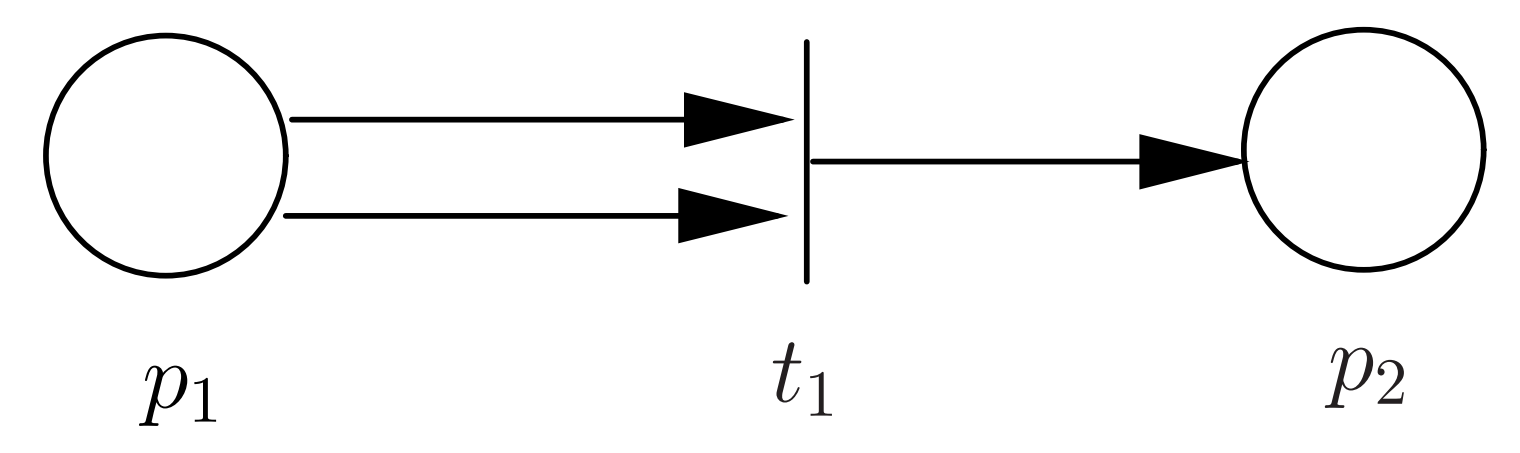
\includegraphics[scale=0.3]{exemplo_simples_rede_petri.png}
	\caption[Rede de Petri Simples]{Rede de Petri Simples. Fonte: \textcite{CassandrasLafortune08}.}
	\label{fig:rede_petri_simples_ex_01}
\end{figure} 

Para a mudança de estado dessa representação é necessário, no mínimo, duas marcações no lugar $p_{1}$. Com essa condição satisfeita, a transição $t_{1}$ passa a estar habilitada, tornando possível a mudança de estado, como ilustrado na figura \ref{fig:rede_petri_simples_ex_02}.

\newpage

\begin{figure}[ht] 
	\centering
	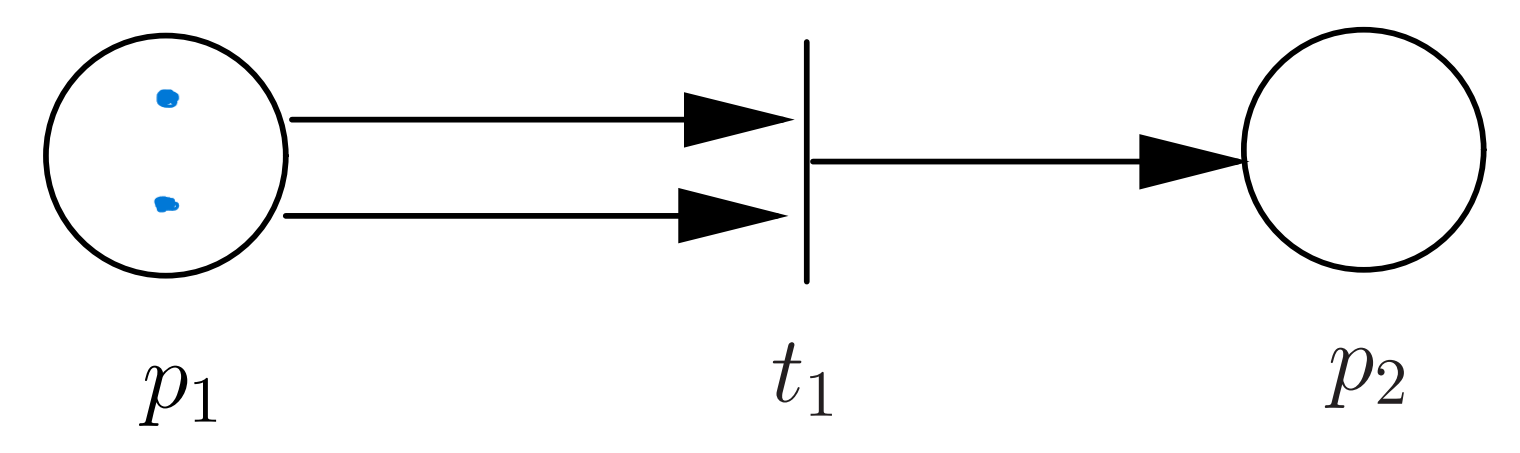
\includegraphics[scale=0.3]{exemplo_simples_rede_petri_marcacao_p1.png}
	\caption[Rede de Petri Simples]{Transição $t_{1}$ habilitada. Fonte: \textcite{CassandrasLafortune08}.}
	\label{fig:rede_petri_simples_ex_02}
\end{figure}

Após a execução da transição $t_{1}$, as duas marcações em $p_{1}$ somem, e uma marcação em $p_{2}$ surge. Essa lógica se dá por meio do peso dos arcos. O arco $(p_{1},t_{1})$, anterior a transição $t_{1}$ possui peso 2, logo o lugar $p_{1}$ cede duas marcações para a transição $t_{1}$ ocorrer. De forma análoga, o lugar $p_{2}$ ganha uma marcação, pois o arco $(t_{1},p_{2})$, posterior a transição $t_{1}$, tem peso igual a 1. Essa lógica é ilustrada pela figura \ref{fig:rede_petri_simples_ex_03}.

\begin{figure}[ht] 
	\centering
	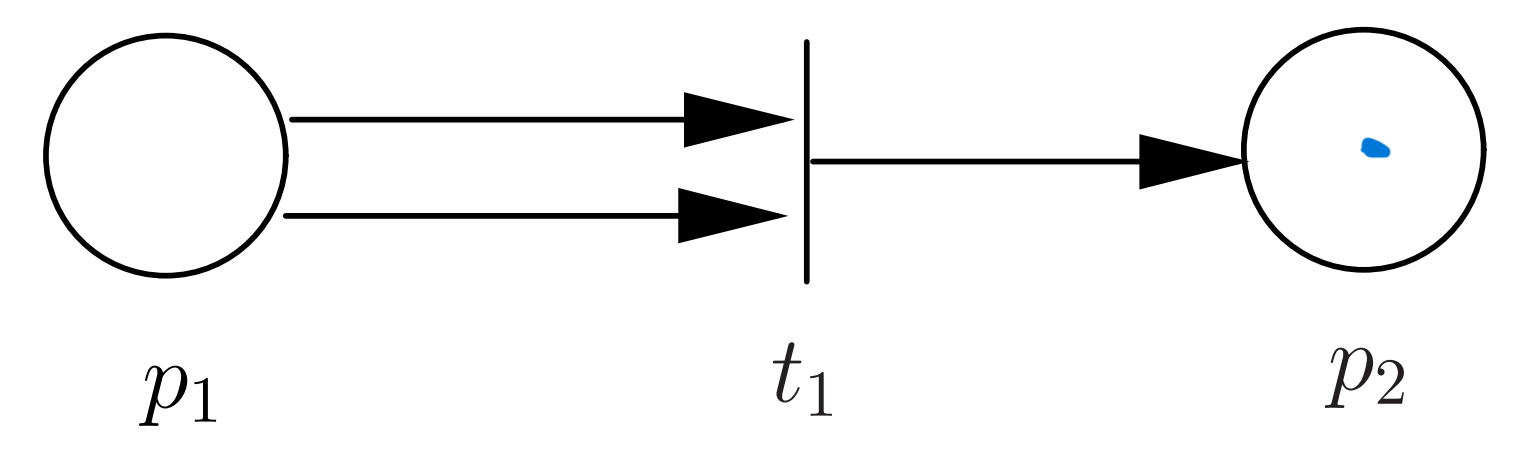
\includegraphics[scale=0.3]{exemplo_simples_rede_petri_marcacao_p2.png}
	\caption[Rede de Petri Simples]{Rede de Petri após a transição $t_{1}$ ter sido executada. Fonte: \textcite{CassandrasLafortune08}.}
	\label{fig:rede_petri_simples_ex_03}
\end{figure}

%\end{exemplo}

Com o exemplo \ref{exemplo_rede_petri_simples}, é possível entender o princípio básico de funcionamento das redes de Petri. Dessa forma, tem-se que:

 \begin{enumerate}[label=(\alph*)]
    \item \textbf{habilitação de uma transição:} para a habilitação de uma transição $t_{i}$ é necessário que o número de marcações associados ao lugar $p_{i}$, anterior a transição, seja igual, ou superior, ao peso do arco que conecta o lugar $p_{i}$ a transição $t_{i}$;
    \item \textbf{peso dos arcos:} ...;
    \item \textbf{movimentação das marcações:} ....
\end{enumerate}


\begin{exemplo} \textbf{Uma rede de Petri mais desenvolvida}
\label{exemplo_rede_petri_desenvolvidada}

\end{exemplo}

A lógica utilizada nas redes de Petri podem facilmente ser traduzidas para os modelos utilizados na lógica de programação Ladder, uma vez que as redes de Petri também se utilizam da álgebra booleana. 

%\begin{exemplo} \textbf{A mesma representação em rede de Petri e Lader}
    
%\end{exemplo}

% \textcolor{red}{Trocar imagens das redes de Petri por imagens retiradas da minha própria aplicação.}

\subsection*{Variantes das redes de Petri clássica}

Além da rede de Petri clássica, com o passar dos anos, e com o avanço da tecnologia, houve a necessidade de se adaptar as redes de Petri para atender cenários mais realistas e completos. A partir dessas variações, três delas se destacam, sendo elas as redes de Petri Temporizadas \ref{exemplo_temporarizada}, Coloridas \ref{exemplo_colorida} e Estocásticas \ref{exemplo_estocastica}. Cada uma delas, permite uma representação mais abrangente dos sistemas do mundo real, pois permitem o desenvolvimento de aspectos como tempo, características distintas e incertezas que compõem os diversos tipos de sistemas.


\subsubsection*{Temporizada}

\textcolor{red}{referenciar o artigo dcce.ibilce.unesp.br/~aleardo/cursos/str/cap3.pdf }

As redes de Petri Temporizadas surgiram a partir da necessidade de se atribuir uma propriedade temporal a certos atributos de um sistema. Ao contrário das redes de Petri clássicas, que consideram as transições como instantâneas, as redes de Petri Temporizadas reconhecem que uma vasta quantidade de sistemas do mundo real estão intrinsecamente ligados a variáveis de tempo. Tal fato é extremamente relevante, já que a maiorias dos eventos nesses sistemas demanda certo período de tempo para sua execução completa.

Nas redes de Petri Temporizadas, pode-se considerar dois cenários para a associação de variáveis de tempo. No primeiro cenário, se tem a associação de tempo $C_{i}$ a duração de uma certa transição $t_{i}$. Ou seja, o evento representado pela transição terá um intervalo de tempo para ser executado. No segundo cenário, associa-se a variável de tempo $C_{i}$ aos lugares $p_{i}$. Dessa forma, as marcações tornam-se disponíveis apenas após o intervalo de tempo. Define-se assim: 

\begin{itemize}
        \item Tempo $C_{i}$ associado a transição $t_{i}$;
        \item Tempo $C_{i}$ associado ao lugar $p_{i}$.
\end{itemize}

As transições temporizadas, nos modelos gráficos, para se diferenciar das transições instantâneas, possuem uma cor associada diferente, e isso pode ser evidenciado na maioria dos softwares já disponíveis. Enquanto as transições instantâneas possuem fundo preto, as transições temporárias possuem fundo branco. Além disso, quando uma transição estiver disponível para o disparo, ela possuirá fundo vermelho, conforme a figura \ref{fig:cores_transição}. 

\begin{figure}[ht] 
	\centering
	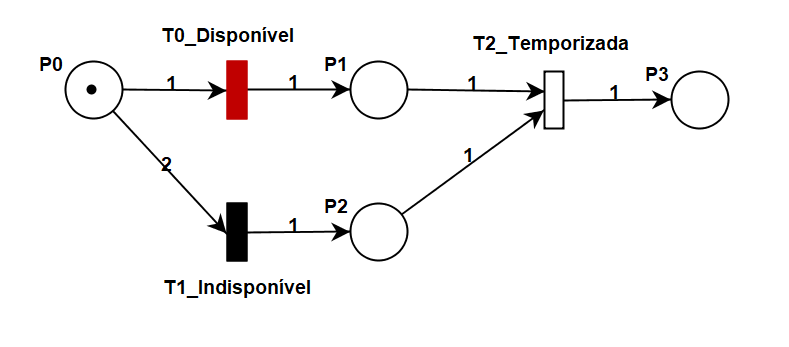
\includegraphics[scale=0.75]{figuras/exemplo_cores_transicao.png}
	\caption[Cores dos tipos de transição]{Cores dos tipos de transição. Fonte: Pipe.}
	\label{fig:cores_transição}
\end{figure}

No exemplo \ref{exemplo_temporarizada} há uma transição fonte $t_{0}$, que está sempre habilitada, ligada a posição $p_{0}$. O lugar $p_{0}$ está ligado a uma transição temporizada $t_{1}$, por meio de um arco $w(p_{0},t_{1})$ de peso 2. Além disso, a transição $t_{1}$ possui um tempo $C_{1}$ associado. Ou seja, após o disparo da transição $t_{1}$, haverá um tempo $C_{1}$ de espera, indicando o tempo de execução do evento associado a transição. Após a decorrência desse tempo, duas marcações, associadas ao lugar $p_{0}$, se transformarão em apenas uma marcação no lugar $p_{1}$.  

\begin{exemplo} \textbf{Temporizada}
\label{exemplo_temporarizada}

\begin{figure}[ht] 
	\centering
	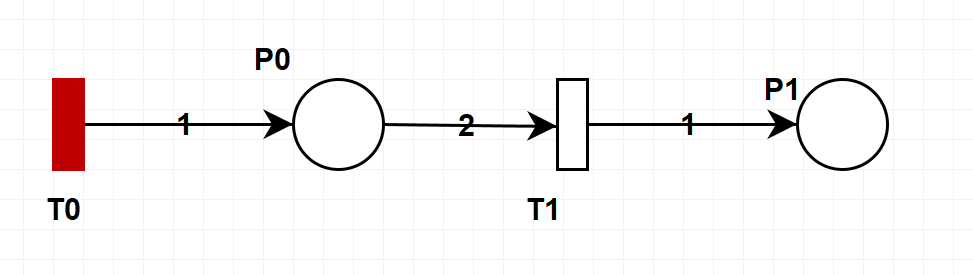
\includegraphics[scale=0.55]{figuras/exemplo_rede_petri_temporizada_1.png}
	\caption[Rede de Petri Temporizada - Estágio 1]{Rede de Petri Temporizada - Estágio 1. Fonte: Pipe.}
	\label{fig:rede_petri_temporizada_ex_01}
\end{figure}

\begin{figure}[ht] 
	\centering
	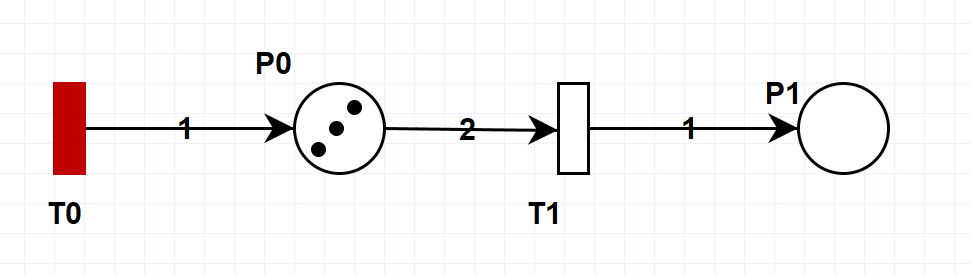
\includegraphics[scale=0.55]{figuras/exemplo_rede_petri_temporizada_2.png}
	\caption[Rede de Petri Temporizada - Estágio 2]{Rede de Petri Temporizada - Estágio 2. Fonte: Pipe.}
	\label{fig:rede_petri_temporizada_ex_02}
\end{figure}

\begin{figure}[ht] 
	\centering
	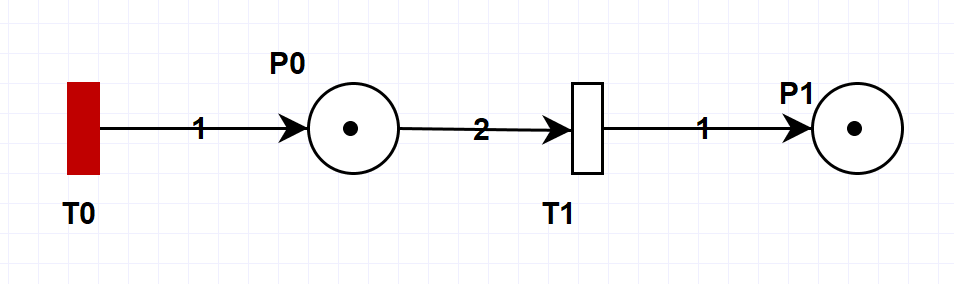
\includegraphics[scale=0.55]{figuras/exemplo_rede_petri_temporizada_3.png}
	\caption[Rede de Petri Temporizada - Estágio 3]{Rede de Petri Temporizada - Estágio 3. Fonte: Pipe.}
	\label{fig:rede_petri_temporizada_ex_03}
\end{figure}

\end{exemplo}

\subsubsection*{Colorida}

As redes de Petri Coloridas surgiram com a ideia de diminuir o tamanho das representações \cite{frances2003introduccao}, uma vez que muitas representações contam com ideias semelhantes. Através da individualização das marcações, os processos e recursos de um sistema podem agora representar diferentes ideias em uma mesma rede, ou parte dela. O termo "colorida" surge da ideia de termos marcações, com diferentes cores, representando diferentes recursos. Essa forma de representação tem como principal benefício reduzir o tamanho e, consequentemente, a complexidade da representação em uma rede de Petri. Comparando os exemplos, consegue-se analisar tal propriedade. Ambas as redes representam a mesma ideia, porém na segunda representação temos uma quantidade menor de elementos, o que facilita o entendimento. 

Uma vez que se consegue representar as marcações com diferentes cores, torna-se mais simples a representação de sistemas complexos, diminuindo a complexidade das análises. Nas redes de Petri tradicionais, cada lugar representa um único estado do sistema representado. As redes de Petri coloridas deixam de forma mais intuitiva e clara a representação de múltiplos estados ou recursos. 

\begin{exemplo} \textbf{Colorida}
\label{exemplo_colorida}

\end{exemplo}

\subsubsection*{Estocásticas}

Uma rede de Petri estocástica é mais uma variação das redes de Petri clássicas. Enquanto as redes de Petri clássicas são frequentemente usadas para representar sistemas discretos e determinísticos, as redes de Petri estocásticas permitem incorporar a aleatoriedade e a incerteza na representação.

Nas redes de Petri estocásticas, os elementos básicos, como lugares, transições e arcos, são semelhantes aos das redes de Petri convencionais. No entanto, a principal diferença é que as transições não são ativadas de forma determinística, mas sim com base em probabilidades. Isso significa que a ocorrência de uma transição é governada por um processo estocástico, como um processo de Poisson, e a escolha de qual transição ocorre em um determinado momento é determinada por probabilidades.

Essa abordagem estocástica é especialmente útil para modelar sistemas onde eventos ocorrem de maneira aleatória, como sistemas de comunicação, sistemas biológicos e sistemas de manufatura com variações de tempo e recursos. As redes de Petri estocásticas permitem a análise de propriedades estatísticas do sistema, como a probabilidade de estados específicos serem alcançados ou a distribuição de tempo entre eventos.

Conforme o exemplo \ref{exemplo_estocastica} é possível analisar o funcionamento de uma rede de Petri estocástica.

\textcolor{red}{Criar exemplo de Rede de Petri estocástica}

\begin{exemplo} \textbf{Estocásticas}
\label{exemplo_estocastica}

\end{exemplo}

%\section{Linguagens de marcação de texto}

\section{Tecnologias para o desenvolvimento web}

\subsection*{HTML}

\subsection*{CSS}

\subsection*{JavaScript}

\section{Simuladores Conhecidos}

\subsection*{Pipe}

\subsection*{Online Petri-net simulator - OPN}

\subsection*{TryRdP}

% ---
\chapter{Desenvolvimento} \label{cap:desenvolvimento}

% Caso seja um trabalho oriundo da Escola de Minas ou do ICEB, é conveniente apresentar uma fórmula:
% \begin{equation}
% f(x) = \int \limits_{0}^{+ \infty} \tanh \left[\ln (j \omega)^2 \right] dx \,. \label{eq:01}
% \end{equation}

% Lembre-se: equações fazem parte do texto e, por isso, devem ser pontuadas! Assim, conforme a equação \eqref{eq:02}, que está na página \pageref{eq:02}, tem-se uma demonstração. Um outro exemplo é :
% \begin{equation}
% \lim\limits_{x \to 0} \frac{\sin (x)}{x} = 1 \,. 
% \label{eq:02}
% \end{equation}

% Pode-se também escrever equações na linha, como $E = m c^2\,,$ mas somente para expressões menores.

% Se for desenvolvido no ICHS (ver figura \ref{fig:309}), tem-se uma noção melhor do movimento estudantil. A figura \ref{fig:308} ilustra bem o fato.

% % uma figura
% \begin{figure}[h] % o ``h'' significa colocar a figura aqui (here)
% 	\centering
% 	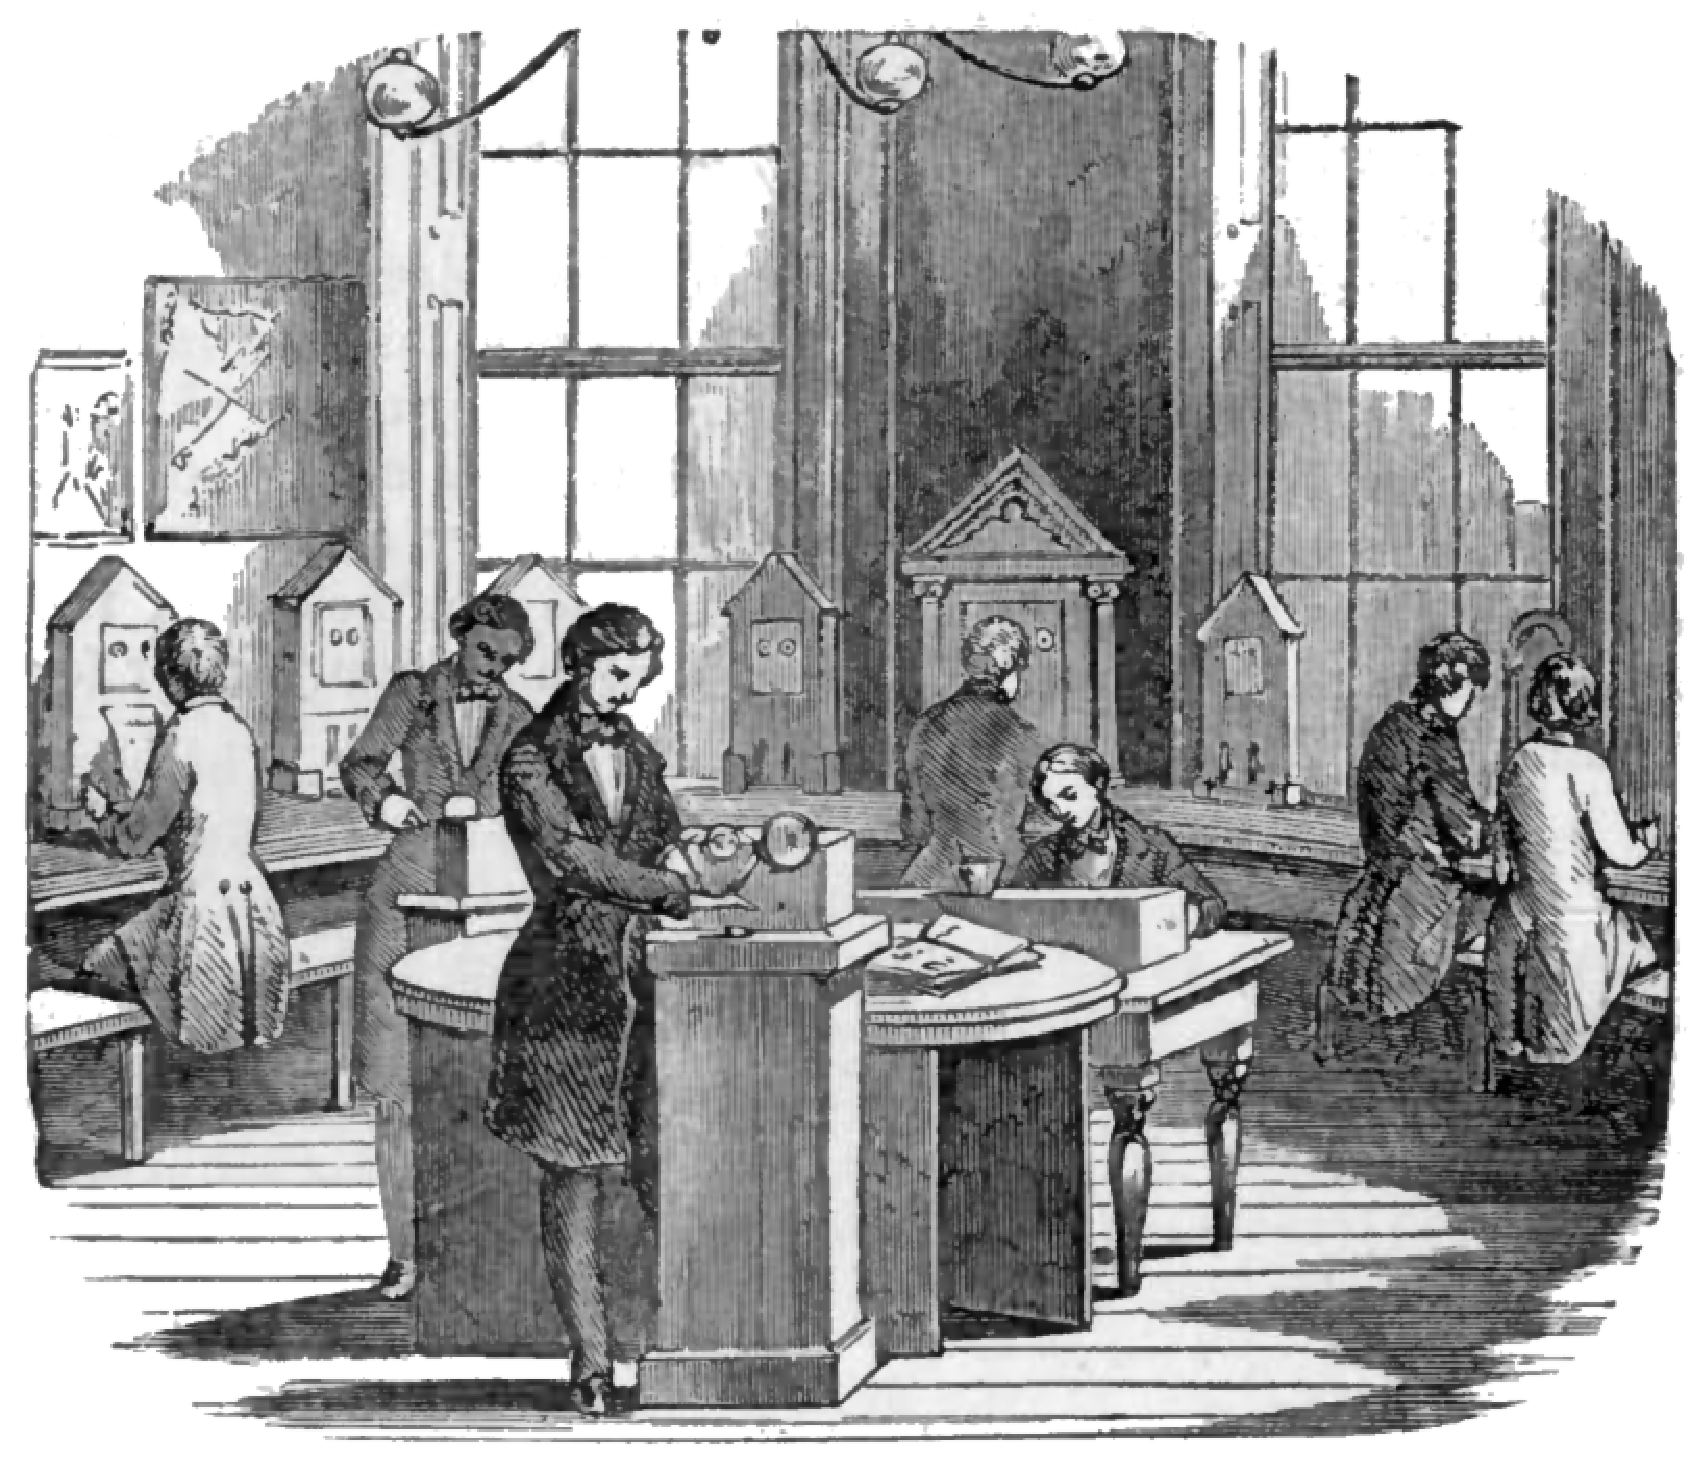
\includegraphics[scale=0.3]{fig09.pdf} % teste os valores
% 	\caption[Legenda reduzida. Aparece apenas no sumário]{Legenda completa - não aparece no sumário. Aqui você pode colocar uma explicação melhor. Fonte: \textcite{boyle1772}.}
% 	\label{fig:308}
% \end{figure}

% \lipsum[22]

% % uma figura
% \begin{figure}[h]
% 	\centering
% 	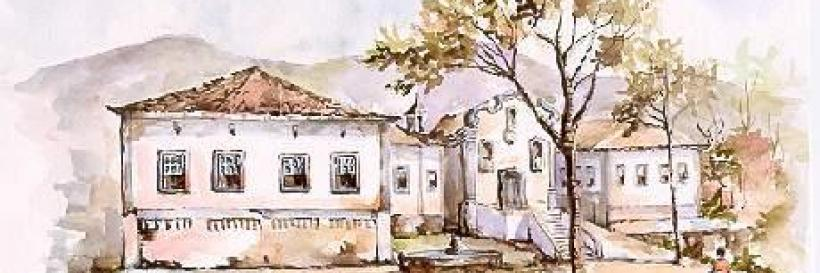
\includegraphics[scale=0.4]{ichs2.jpg} % teste os valores
% 	\caption[Legenda reduzida - aparece apenas no sumário]{Legenda completa - não aparece no sumário. Aqui você pode colocar uma explicação melhor, sem que ela apareça no sumário do seu trabalho. Fonte: \cite[p.~117]{boyle1772}.}
% 	\label{fig:309}
% \end{figure}



% \section{Uma seção extravagante}
% % ---
% \lipsum[21]


% % primeiro capitulo de Resultados
\chapter{Considerações Finais} \label{cap:resultados}
% % ---

% Neste capítulo é apresentada uma análise dos resultados obtidos.

% \section{Dados, dados, dados}
% % ---
% \lipsum[21]

% % ----------------------------------------------------------
% %\phantompart
% % Insere arquivo de Considerações Finais ou Conclusões
% \chapter{Considerações finais}
% As últimas palavras podem ser apresentadas neste capítulo. Ele pode ser numerado ou não. Caso queria que ele não possua numeração, utilize \* apos o comando chapter.

% \lipsum[21]

% ----------------------------------------------------------
% ELEMENTOS PÓS-TEXTUAIS
% ----------------------------------------------------------
\postextual
% ----------------------------------------------------------

%% ----------------------------------------------------------
%% Referências bibliográficas
%% ----------------------------------------------------------
% toca nome de bibliografia para ``Referências''
\printbibliography%[title=Referências]

% ----------------------------------------------------------
% Glossário
% ----------------------------------------------------------

% Consulte o manual da classe abntex2 para orientações sobre o glossário.

% \glossary

% ----------------------------------------------------------
% Apêndices
% ----------------------------------------------------------
%(Lembre-se: Apendices são de autoria do próprio autor do texto.
% Anexos são elementos de autorias de outros, que o autor do texto julga interessante apresentar)
% ---
% Inicia os apêndices:
% ---
% \begin{apendicesenv}

% % Imprime uma página indicando o início dos apêndices
% %\partapendices
% % ---
% % Insere arquivo com o apêndice A
% % --------

% \chapter{libero justo}
% Lembre-se: apêndices são de autoria do próprio autor do texto. Anexos são elementos de autorias de outros, que o autor do texto julga interessante apresentar


% \end{apendicesenv}
% % ---

% % ----------------------------------------------------------
% % Anexos
% % ----------------------------------------------------------
% %(Lembre-se: Apendices são de autoria do próprio autor do texto.
% % Anexos são elementos de autorias de outros, que o autor do texto julga interessante apresentar)
% % ---
% % Inicia os anexos
% % ---
% \begin{anexosenv}

% % Imprime uma página indicando o início dos anexos
% %\partanexos

% % ---
% % Insere arquivo com os anexos 1, 2
% \chapter{Morbi ultrices rutrum lorem.}
% Lembre-se: apêndices são de autoria do próprio autor do texto. Anexos são elementos de autorias de outros, que o autor do texto julga interessante apresentar

% \chapter{Lorem Morbi ultrices rutrum.}
% Lembre-se: apêndices são de autoria do próprio autor do texto. Anexos são elementos de autorias de outros, que o autor do texto julga interessante apresentar

% % ---
% \end{anexosenv}

% %---------------------------------------------------------------------
% % INDICE REMISSIVO
% %---------------------------------------------------------------------
% %\phantompart
% \printindex
% %---------------------------------------------------------------------

\end{document}